\section{Integraltransformationen}

\subsubsection*{Faltung}

$$y(t) = (x_1 * x_2)(t) = \int \limits _{-infty} ^{infty} x_1(\tau) \cdot x_2(t-\tau) d\tau$$
\textbf{Eigenschaften:}
\begin{itemize}
  \item Kommutativ ($f * g = g * f$)
  \item Assoziatiov ($(f*(g*h)) = ((f*g)*h)$)
  \item Distributiv ($f*(g+h)= f*g + f*h$)
\end{itemize}

\subsection{Fourier-Reihe und Transformation}
\subsubsection*{Fourier-Reihe}
\begin{tabular}{p{4.5cm}p{14.5cm}}
  Trigonometrische Form &
  $x(t) = \frac{u_0}{2} + \sum \limits _{n = 1} ^{\infty} u_n \cdot cos(2\pi n f_0 \cdot t) + v_n \cdot sin(2\pi n f_0 \cdot t) $
  \newline $u_n = \frac{2}{T} \int \limits _{T} x(t) \cdot cos(2\pi n f_0 \cdot t)dt$
  \newline $v_n = \frac{2}{T} \int \limits _{T} x(t) \cdot sin(2\pi n f_0 \cdot t)dt$
  \\
  \\
  Harmonische Form      &
  $x(t) = r_0 + \sum \limits _{n = 1} ^{\infty} r_n \cdot cos(2\pi n f_0 \cdot t + \varpi_n)$
  \newline $r_0 = \frac{u_0}{2} = \frac{1}{T} \int  \limits _{T} x(t) dt $
  $r_n > 0 = \sqrt{u_n^2 + v_n^2}$
  $\varphi = arg(u_n - j \cdot v_n) $
  \\
  \\
  Komplexe Form         &
  $x(t) = \sum \limits _{n= -\infty} ^{\infty} c_n \cdot e^{jn2\pi f_0 \cdot t}$
  \newline $c_n =\overline{c_{-n}} = \frac{1}{T} \int \limits _{0} ^{T} x(t) \cdot e^{-j n 2 \pi f_0 \cdot t} dt$
  \newline $ 2\pi f_0$ wird auch als \textbf{Kreisfrequenz}  $\omega$ bezeichnet, \newline $f_0$ = Frequenz des Grundsignals $x(t)$. 
  \\
  \\
  Umrechnung Koeffizienten &
  $c_n =\overline{c_{-n}} = \frac{a_n - jb_n}{2} (n = 0,1,2,3,..., b_0 =0)$
  \newline $a_n = 2 \cdot Re(c_n); \; b_n = -2 \cdot Im(c_n) (n = 0,1,2,3,..., b_0 =0)$\\
\end{tabular}

\begin{multicols}{2}
  
  \subsubsection*{Fouriertransformation $\mathcal{F}(\omega)$}
  $$ X(\omega) = \mathcal{F}[x(t)] = \int \limits _{-\infty} ^{+\infty} x(t) \cdot e^{-j \omega t} dt $$
  $$ x(t) = \mathcal{F}^{-1}[X(\omega)] = \frac{1}{2 \pi} \int \limits _{- \infty} ^{+ \infty} X(\omega) \cdot e^{j \omega t} d\omega$$
  
  \subsubsection*{Spektraldarstellung}
  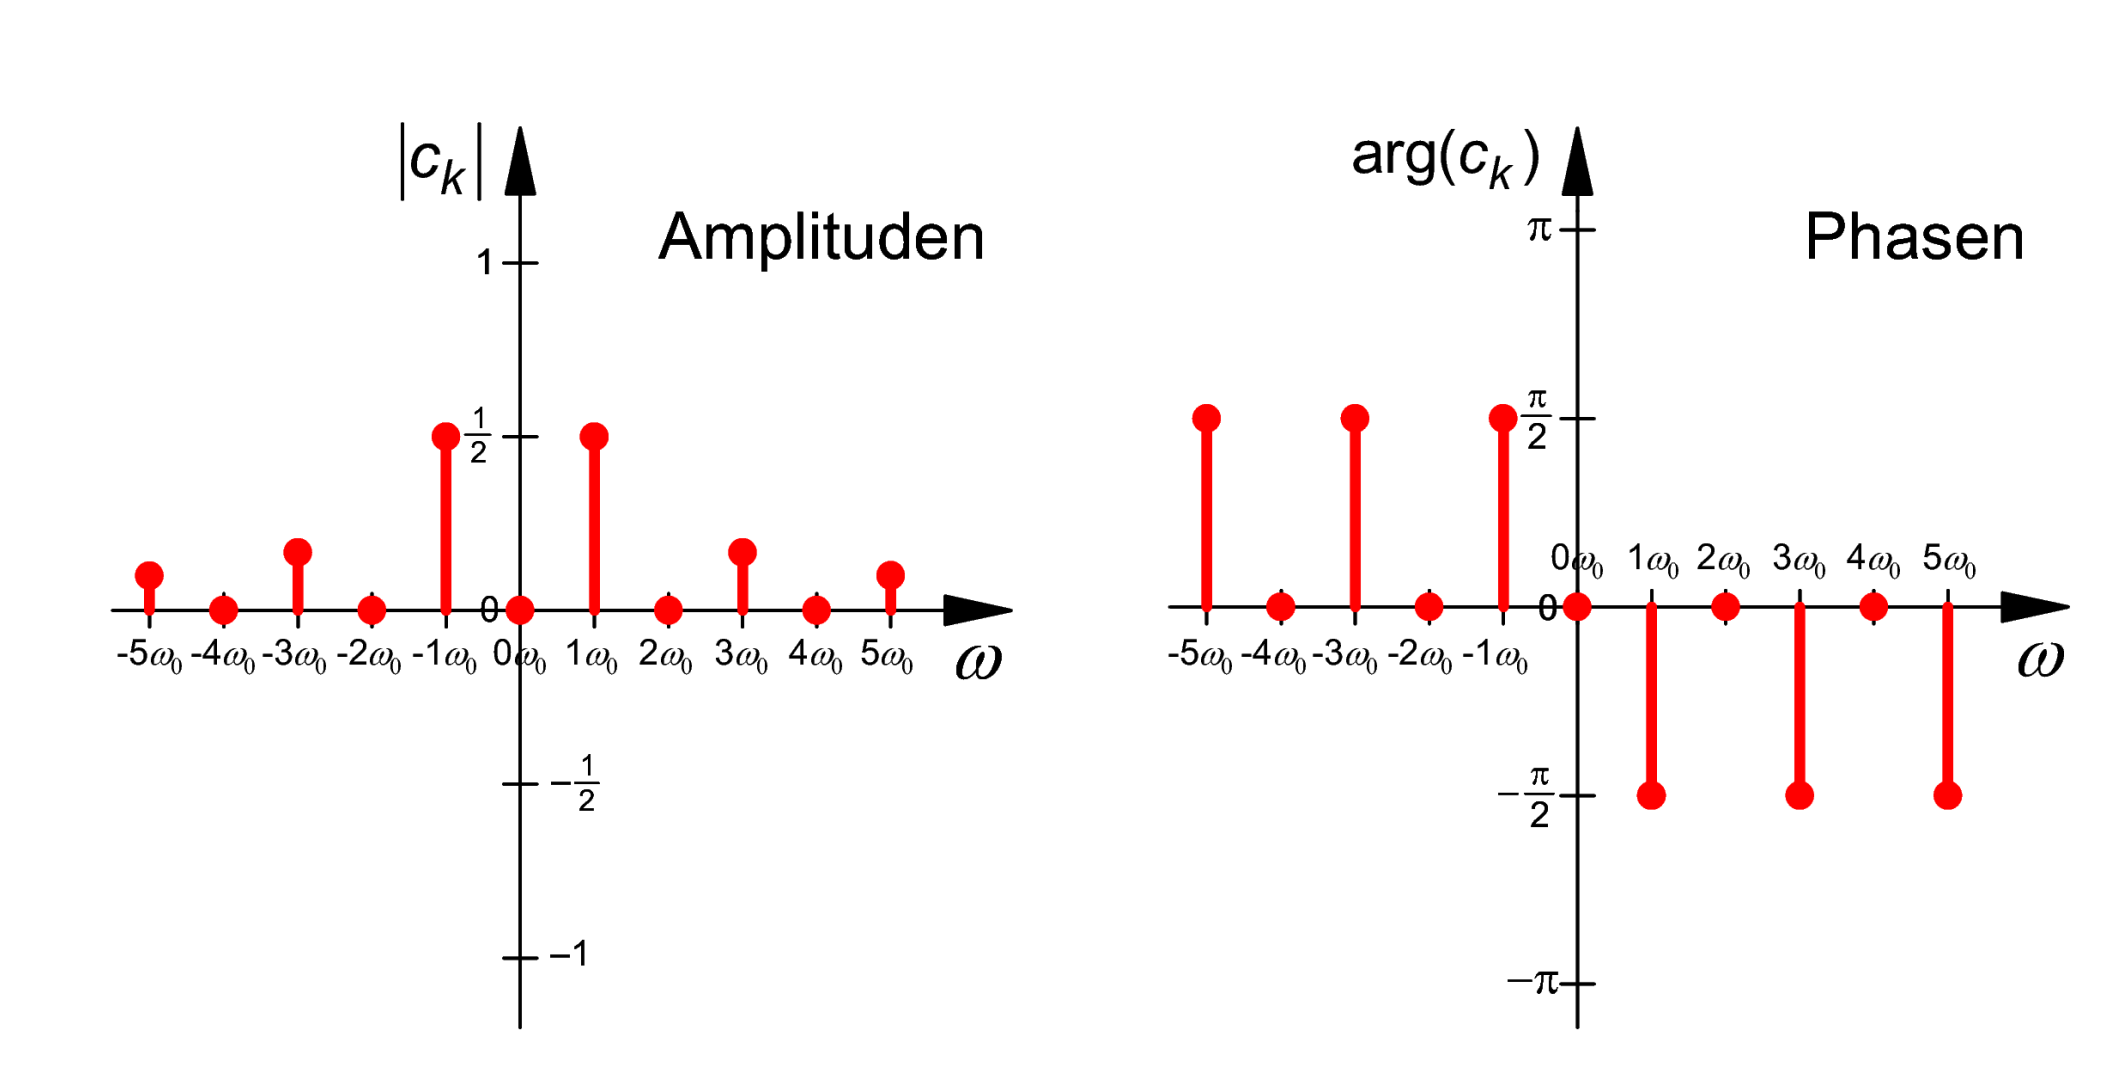
\includegraphics[width = 6cm]{include/Integraltransformationen/img/Spektrum.png}
\end{multicols}

\subsection{Laplace-Transformation}
TODO: %LAPLAAAAAAAAACEEEE

\subsection{Hilbert-Transformation}
Hilbert Transformation ist die Anwendung eines Quadraturfilters. \\
Definition im \textbf{Zeitbereich:}
$$\hat{x}(t) = x(t) * \frac{1}{\pi t} = \frac{1}{\pi} \int \limits _{-\infty} ^{\infty} \frac{x(\tau)}{t-\tau} d\tau$$
Im \textbf{Frequenzbereich}:
$$\hat{X}(\omega) = X(\omega) \cdot H(\omega) = -j \cdot sgn(\omega) \cdot X(\omega)$$
